% $  Id: validation.tex  $
% !TEX root = main.tex


%%
\section{Validation}
\label{sec:validation}

To validate the appropriateness of CollabIDE, we define two research questions:
\begin{enumerate*}[label=(\arabic*)]
\item Does an automated \ac{VCS} improve productivity in software development?
\item Is it possible to use software versions to generate multiple software variants from a product?
\end{enumerate*} 
To answer these questions, we conducted an empirical evaluation 
to measure how effective CollabIDE was at reducing overhead problems 
in both Distributed Software Development and Software Product Lines.

%%%%
\subsection{Experiment Design}

\authorcomment[missing]{NC}{Context, Research questions, analysis method, data collection method}

We designed an isolated experiment for each question. In each experiment, we asked 
a group of developers to solve programming tasks using either CollabIDE or a 
conventional IDE following a set of instructions that aimed to emulate the workflow of each development model. The experiments differed in team sizes, the required tasks to complete and the instructions assigned to each group. Two measures were taken in each experiment, first, the completion percentage of the total tasks assigned and second, the amount of time in minutes spent performing actions related to version control. The analysis of these measures would then enable us to answer the proposed questions.

%%%%
\subsubsection{Experiment 1: Software development in a distributed set-up}
The objective of this experiment was mainly to quantify the overhead reduction that can be achieved when using CollabIDE in a distributed set-up in order to answer the first research question. For the experiment, groups of developers had to implement a set of common graph algorithms using only JavaScript. The specific instruction they had to follow was that they needed to use version control periodically so that both team members code remained up to date with their partner's changes through the experiment. 


%%%%
\subsubsection{Experiment 2: Product variants development and deployment}
In this second experiment the objective was to also quantify the overhead reduction that can be achieved with CollabIDE in a product lines set-up, this time to answer our first and second research question. In this case, the programming task was to implement a set of data structures with basic functionality using JavaScript  or Java. Each data structure also had to be a variant of a given base data structure. Participants had to use version control to manage the different product variants that were involved in the programming tasks.

%%%%
\subsection{Experiment Setup}

Six developers were gathered for the first experiment, then they were split into groups of two. Two groups would be using CollabIDE and the remaining group would be using Sublime Text in conjunction with git and github. The participants were given a total of 90 minutes to accomplish this task. Each group was required to obtain their partner’s changes every fifteen minutes using their tools at hand. In the Software Product Lines experiment, a different group of four developers was gathered. Two of them would be using CollabIDE and the other two would be using Eclipse in conjunction with git and github. These participants were also given 90 minutes to complete their task. For experiment 2, There was no constraint in how often participants needed to use version control.


\authorcomment[missing]{NC}{Tools, exercise}
	

%%%%
\subsection{Results}

In this section we analyze the results of each experiment, specifically how each measure taken helps us tell if there was an increase in productivity.

\subsubsection{Experiment 1 Results}

First, in \fref{fig:resultsCollaborative} we show the results for each group and the background of each participant. Both groups that used CollabIDE achieved a higher completion rate (on average of 11 percent more tasks completed) than the control group (\fref{fig:completionCollaborative}). On top of that, they also spent significantly less time performing actions related to version control (an average of 33.2 less minutes) (\fref{fig:versionControlCollaborative}). The higher completion rate achieved by the groups that used CollabIDE can be attributed to the fact that the developers could spend more time coding as they didn’t have to invest much time in version control. It is clear why there is such a significant difference in time for both IDEs results. While the control group had to follow the common git workflow of committing, pushing, pulling changes and solving the possible conflicts that could arise, the CollabIDE groups could avoid this process altogether as CollabIDE’s features ensured that both team members always had each other latest changes without conflicts. Thus, the only action they needed to perform was creating a new version using the side menu of CollabIDE.


When analyzing the developers background, one factor that could have influenced the results is the fact that all of the participants that used CollabIDE had more experience in both Javascript and distributed development. Nevertheless, the experiment was designed in a way that only a basic knowledge of Javascript and data structures was required so the results were most likely not influenced by this.

\begin{figure}[htbp]
  \centering
  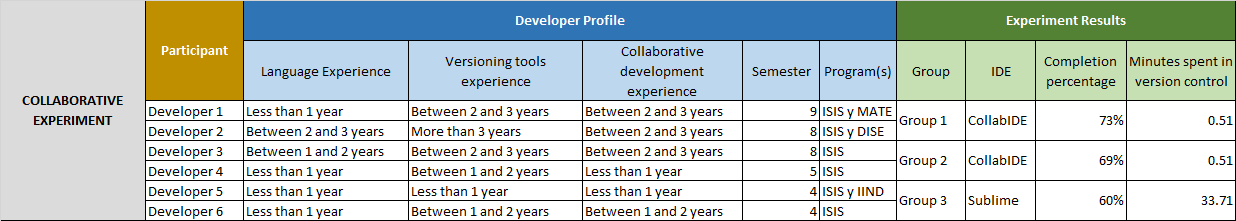
\includegraphics[width=1\textwidth]{img/resultsTableCollaborative}
  \caption{Distributed Development experiment results}
  \label{fig:resultsTableCollaborative}
\end{figure}

\begin{figure}[htbp]
  \centering
  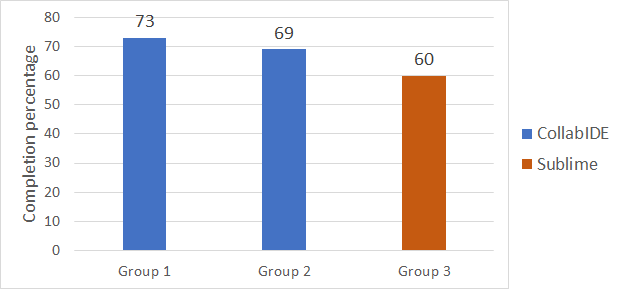
\includegraphics[width=0.8\textwidth]{img/completionCollaborative}
  \caption{Completion percentage graph for Distributed Development}
  \label{fig:completionCollaborative}
\end{figure}

\begin{figure}[htbp]
  \centering
  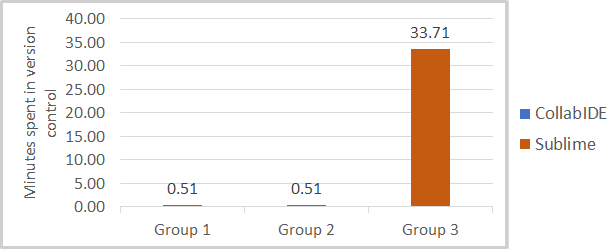
\includegraphics[width=0.8\textwidth]{img/versionControlCollaborative}
  \caption{Time spent in version control graph for Distributed Development}
  \label{fig:{img/versionControlCollaborative}}
\end{figure}

\subsubsection{Experiment 2 Results}

In \fref{fig:resultsTableProductLine} we show the results and background for each developer in the product line development experiment. Like the first experiment, the developers that employed CollabIDE obtained better results, but in this case, the difference between using one IDE versus using the other was not very significative. With CollabIDE, the developers finished on average 4 percent more tasks (\fref{fig:completionProductLine}) and spent 2.83 less minutes in version control than the developers using Eclipse (\fref{fig:versionControlProductLine}).The process of creating new product variants and their respective functionalities varied significantly in each IDE. With Eclipse and git, participants had to create a branch for each variant and then checkout between branches when they needed to work on a variant’s specific code. On the other hand, with CollabIDE, participants needed to first create a product version for each variant, then, for each variant create a new developer. This way the participants could take advantage of code highlighting, showing and hiding to easily distinguish which code fragments belonged to which variant. Thus, while Eclipse and Git makes variant creation straightforward, the process of switching between them isn’t as smooth. The contrary happens with CollabIDE where creating a variant is a longer process but switching between them is faster. According to this, it makes sense that in the results there wasn’t that big of a difference as there is a tradeoff when using one IDE versus the other. However, in real life contexts, projects usually take longer to complete and variant switching operations are more plentiful than variant creating ones. Therefore, in a real life context CollabIDE would provide better productivity for a development team.


When analyzing other factors that could have influenced the experiment, we found some with a potential impact on the results. First, the tasks needed to be implemented in differentes languages, the differences between languages could hadve lead to some developers having an easier time than others. Another outcome worth mentioning is that one of the developers had problems pushing his changes to github, and at the end of the experiment he only had one branch, meaning he lost the changes he made to various product variants. This occurrence helps reinforce our claim that even using version control systems can harm the productivity of a development team.   
\begin{figure}[htbp]
  \centering
  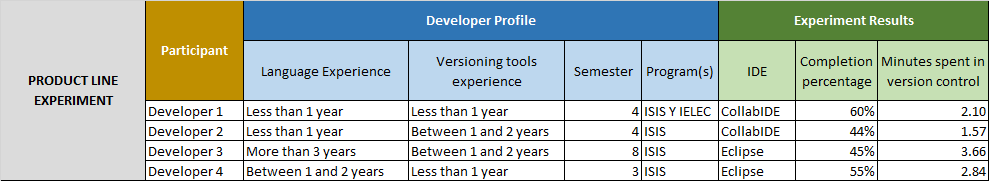
\includegraphics[width=1\textwidth]{img/resultsTableProductLine}
  \caption{Product Line Development experiment results}
  \label{fig:resultsTableProductLine}
\end{figure}

\begin{figure}[htbp]
  \centering
  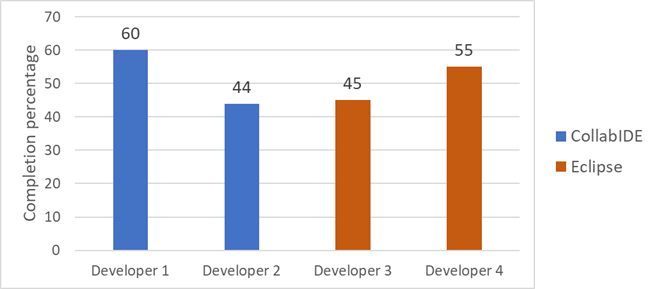
\includegraphics[width=0.8\textwidth]{img/completionProductLine}
  \caption{Completion percentage graph for Product Line Development}
  \label{fig:completionProductLine}
\end{figure}

\begin{figure}[htbp]
  \centering
  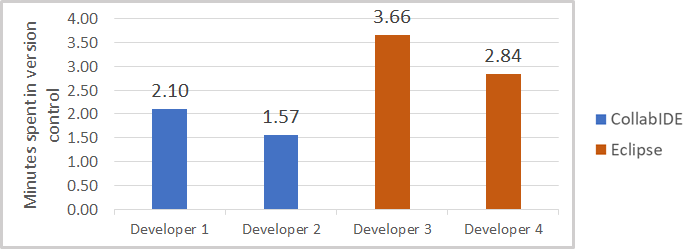
\includegraphics[width=0.8\textwidth]{img/versionControlProductLine}
  \caption{Time spent in version control graph for Product Line Development}
  \label{fig:versionControlProductLine}
\end{figure}

\subsubsection{Survey}
At the end of the experiment, we asked the partipants that used CollabIDE their opinion on the tool's main features. All of them agreed that concurrent programming was easy to understand and that it was of great help in completing their tasks. Version management recieved mixed results as participants though it wasn't too complex but not all of them felt this feature helped them during development. Finally, most participants found the product variant management feature useful and easy to use. Overall, the shared opinion is that CollabIDE was intuitive to use and in most cases, its functionallities let participants solve the programming tasks in an efficent manner. 

%%%%
\subsection{Threats to Validity}
In this section we discuss some aspects of the experiments that can put at risk the validity of the results discussed previously. The first one is that the subject sample size is small, having only one control group in the first experiment and two in the second. Small sample sizes can easily lead to bias [REF], and, in this case, the bias would be towards CollabIDE performing better. Another aspect that can be considered a threat is the low duration of each experiment. In real life contexts, software projects where version control systems are employed usually take months if not years to complete. Additionally, the time intervals between each version control operation are longer, whereas in the experiment they needed to be performed each fifteen minutes. These lower times could also lead to bias towards one of the IDEs, as the development workflow wasn't completely accurate compared to one carried out in a real life context. 


\endinput
